\documentclass[12pt]{article}

% #################### PREAMBLE ##########################

% Global margins for the document
\usepackage[margin=0.6cm]{geometry}

% Define spacing between paragraphs in the document
\setlength{\parindent}{0.5cm} % default indentation before the first line of a paragraph.
\setlength{\topskip}{0.2cm} % indentation at the begging of the first paragraph of every page.
\setlength{\parskip}{0.3cm} % indentation after every paragraph

% Font configurations:
\usepackage{fontspec}
\setmainfont{FreeSerif}

% Math related packages:
\usepackage{amsmath, amssymb, amsthm}

% Embedding *.jpg abd *.png images
\usepackage{graphicx}
\graphicspath{{data/}{../data/}} % define the path to the images

% Provides an underline command which will break over line ends:
\usepackage{ulem}

% Hyper links to places inside the document:
\usepackage{hyperref}
\hypersetup{
    colorlinks=true,
    % These take rgb values as a fraction of n/255.
    % That is really not how RGB works!
    linkcolor=[rgb]{0.1, 0.2, 1},
    filecolor=[rgb]{0.1, 0.2, 1},
    urlcolor=[rgb]{0.1, 0.2, 1},
    citecolor=[rgb]{0.1, 0.2, 1},
    unicode=true,
}
\urlstyle{same}

% Bibliography:
\usepackage{csquotes}
\usepackage[backend=biber]{biblatex}
\addbibresource{init.bib}

% For inserting loremipsum random text:
\usepackage[pangram]{blindtext}

% Allows adding sub tex files to the main tex file:
\usepackage{subfiles} % Best loaded last in the preamble

% #################### DOCUMENT BEGIN ####################

\begin{document}

\begin{center}
    {\Huge Big Centered Text}
\end{center}

1. Tiny noindent text: \\
{\tiny\noindent\Blindtext[1][1]}

2. Scriptsize text with added additional 4cm indentation, which is then removed -4cm:

\addtolength{\parindent}{4cm}
{\scriptsize\Blindtext[1][1]}
\addtolength{\parindent}{-4cm}

3. Footnotesize flush right text:
\begin{flushright}
{\footnotesize\Blindtext[1][1]}
\end{flushright}

4. Normalsize flus left text:
\begin{flushleft}
{\normalsize\Blindtext[1][1]}
\end{flushleft}

5. large centered text:
\begin{center}
{\large Nisi qui culpa pariatur velit deserunt nulla nulla dolor cillum est do nulla ut. Nisi qui culpa pariatur velit deserunt nulla nulla dolor cillum est do nulla ut.}
\end{center}

6. Large text after 2 newlines (baselineskip) : \\[2\baselineskip]
{\Large Nisi qui culpa pariatur velit deserunt nulla nulla dolor cillum est do nulla ut. Nisi qui culpa pariatur velit deserunt nulla nulla dolor cillum est do nulla ut.}

7. Graphics with set width 0.3 of linewidth:
\begin{center}
    
\includegraphics[width=0.3\linewidth]{sample.png}
\end{center}

\newpage

\tableofcontents
\listoffigures
\listoftables
\setcounter{section}{8}

\newpage

\section{LaTeX includegraphics wrapped in a figure}
\begin{figure}[ht!]
    \centering
    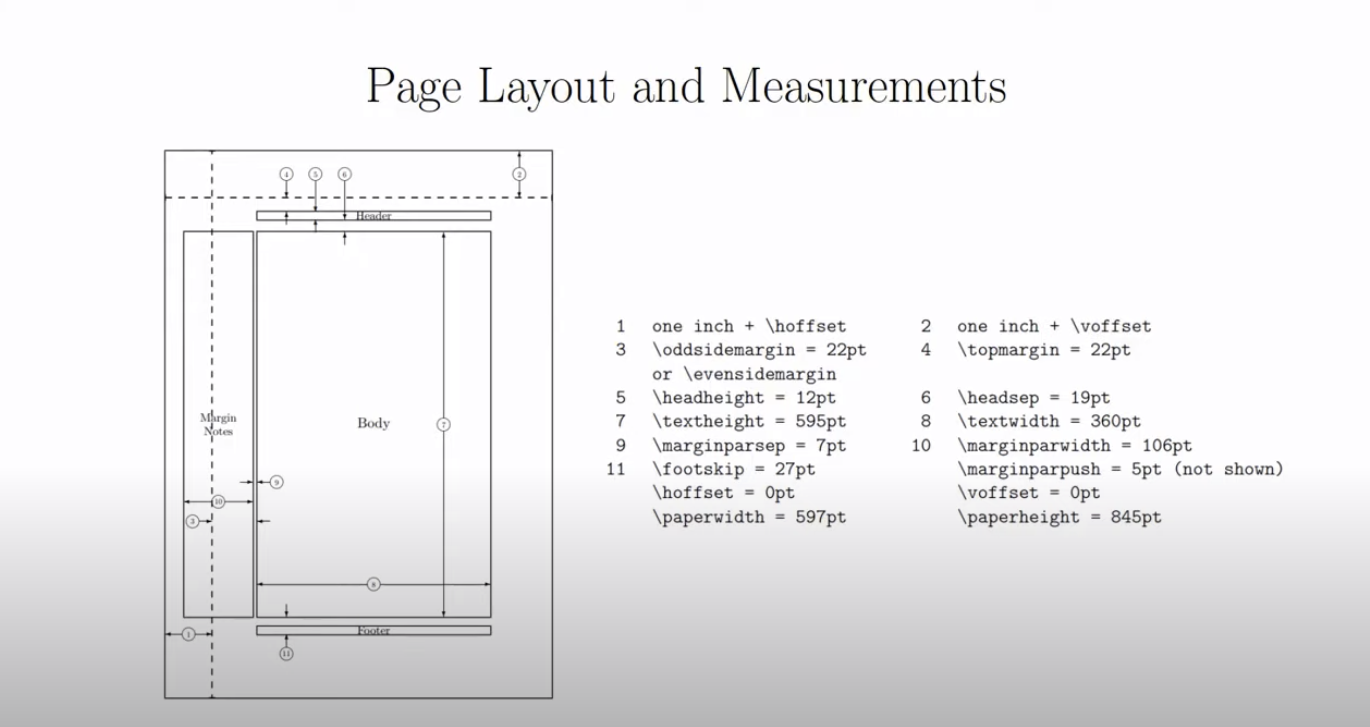
\includegraphics[width=\linewidth]{page_layout.png}
    \caption{LaTeX Page layout and Measurements (width=linewidth)}
    \label{hr_3}
\end{figure}

\section{Section with subsections}

\subsection{LARGE text}
{\LARGE \indent Nisi qui culpa pariatur velit deserunt nulla nulla dolor cillum est do nulla ut. Nisi qui culpa pariatur velit deserunt nulla nulla dolor cillum est do nulla ut.}

\subsection{huge text with bold, italic and standard underline}
{\huge \indent Nisi qui \textbf{culpa} \textit{pariatur} \underline{velit deserunt} nulla nulla dolor cillum est do nulla ut.} \\

\subsection{Huge text with combined bold, italic and standard underline}
{\Huge \indent Nisi qui culpa pariatur velit deserunt \underline{\textbf{\textit{nulla dolor cillum est}}} do nulla ut.} \\

\subsection{This is what happens when you underline long text}
\underline{\textbf{Unerlining a long string of text is kinda hard in latex with the default underline so we can use ulem}. Nisi qui culpa pariatur velit deserunt nulla nulla dolor cillum est do nulla ut. Nisi qui culpa pariatur velit deserunt nulla nulla dolor cillum est do nulla ut.} \\

\subsection{We can fix the above problem with the package ulem using uline}
\uline{\textbf{Same with ulem}. Nisi qui culpa pariatur velit deserunt nulla nulla dolor cillum est do nulla ut. Nisi qui culpa pariatur velit deserunt nulla nulla dolor cillum est do nulla ut.}

{\large \noindent ulem also has \uuline{some other} cool \uwave{underlines}.}

\subfile{sections/example.tex}

\section{Basic Math Equations}

\subsection{Displaystyle math equation}

\begin{equation} % equivalent to $$ .. $$
    \sum_{n=1}^\infty \frac{1}{n^2} = \frac{\pi^2}{6}
\end{equation}

\subsection{Inline math with display style mode}

Ex qui anim eu consequat est excepteur ea est. Exercitation officia pariatur pariatur nostrud. Cillum cillum proident minim officia ex. Aliquip ut officia sit voluptate quis dolor sint proident tempor aliquip qui enim. $ \displaystyle \sum_{n=1}^\infty \frac{1}{n^2} = \frac{\pi^2}{6} $ Elit veniam minim commodo proident do aliqua Lorem sunt ex dolore. Irure adipisicing enim eu velit eiusmod reprehenderit. Sit exercitation minim sunt et.

\subsection{Inline math with text style mode}

Ex qui anim eu consequat est excepteur ea est. Exercitation officia pariatur pariatur nostrud. Cillum cillum proident minim officia ex. Aliquip ut officia sit voluptate quis dolor sint proident tempor aliquip qui enim. $ \textstyle \sum_{n=1}^\infty \frac{1}{n^2} = \frac{\pi^2}{6} $ Elit veniam minim commodo proident do aliqua Lorem sunt ex dolore. Irure adipisicing enim eu velit eiusmod reprehenderit. Sit exercitation minim sunt et.

\subsection{Brakets sizes}

These are a bit unreadable:
\begin{equation*}
    ( \sum_{n=0}^N ( \frac{1}{a + b} )^2 )^2
\end{equation*}

\noindent We can use left and right braket:
\begin{equation*}
    \left( \sum_{n=0}^N \left( \frac{1}{a + b} \right)^2 \right)^2
\end{equation*}

% BIB:
\newpage
\printbibliography

\end{document}